
\documentclass[11pt]{article}

\usepackage{amsmath, amssymb}
\usepackage{geometry}
\usepackage{graphicx}
\usepackage{hyperref}

\geometry{margin=1in}

\title{Triplet Phase Lock: A Minimal Model of Structure, Drift, and Threshold Selection}
\author{Dan Hawkley}
\date{}

\begin{document}

\maketitle

\begin{abstract}
We introduce a minimal computational pipeline demonstrating how global structure persists under perturbation, while local drift emerges and is subsequently filtered by strict alignment thresholds. Using a triplet-based sequence construction, we show that increasing directional drift leads to reduced survival under strict cosine similarity constraints. This provides a minimal, reproducible model showing how local instability translates into selective survival under strict constraints.
\end{abstract}

\section{Overview}

We study a minimal pipeline:

\[
\text{structure} \rightarrow \text{variation} \rightarrow \text{selection}
\]

implemented through three stages:

\begin{itemize}
\item Expand ($\Pi$): global structure
\item Extend ($\pi$): local drift
\item Resist ($\Pi$): threshold filtering
\end{itemize}

\section{Expand}

Define the sequence:

\[
N_k = 24k - 25
\]

Triplets:

\[
T_k = (N_k, N_{k+1}, N_{k+2})
\]

This stage establishes a globally invariant linear structure.

\section{Extend}

Local variation is measured by:

\[
\Delta_k = \|T_{k+1} - T_k\|
\]

and directional change:

\[
\|\hat{d}_{k+1} - \hat{d}_k\|
\]

where $\hat{d}_k$ are normalized step directions.

Perturbations introduce drift while preserving global alignment.

\section{Resist}

Alignment is measured via cosine similarity:

\[
\cos\theta_k = \frac{T_k \cdot R}{\|T_k\|\|R\|}
\]

Two thresholds are considered:

\begin{itemize}
\item Broad: $\cos\theta \geq \frac{1}{\sqrt{2}}$
\item Strict: $\cos\theta \geq 0.9995$
\end{itemize}

\section{Drift--Resistance Relationship}

\begin{figure}[h]
\centering
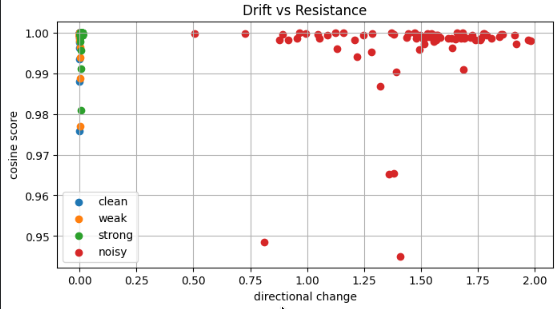
\includegraphics[width=\linewidth]{figures/drift_vs_resistance.png}
\caption{Drift vs Resistance. Each point represents a triplet state. Increasing directional drift produces a measurable drop in cosine alignment under strict thresholds, separating stable and unstable regimes.}
\end{figure}

Combining stages yields:

\[
\text{expand} \rightarrow \text{extend} \rightarrow \text{resist}
\]

Empirical result:

\[
\text{directional drift} \uparrow \;\Rightarrow\; \text{strict resistance} \downarrow
\]

\section{Conclusion}

The system demonstrates:

\begin{itemize}
\item invariant global structure
\item measurable local instability
\item threshold-based survival
\end{itemize}

\[
\text{Structure persists. Drift emerges. Thresholds decide.}
\]

\end{document}
